\chapter{Dos conceitos principais}
\label{cap:main-concepts}

Nesse capítulo, o objetivo é explicitar os conceitos que serão cruciais para a
compreensão do que é dito nos demais capítulos. Como já dito, funciona como
aquela parte do código em que se inclui as bibliotecas e demais arquivos com
definições e módulos e classes e tudo o mais. Tratando desse trabalho, é o
capítulo que garante que o texto estará auto contido na medida do possível, ou
seja, qualquer um que lê-lo, compreenderá o que estiver escrito sem ter que
pesquisar muito fora daqui.

\section{Aventuras de texto}
\label{sec:text-adventure}

Ficção Interativa surge \citep{IF2} das primeiras aventuras de texto. Tal gênero
de jogo surge um pouco antes da década de 70 e consiste em uma espécie de dialogo
entre o jogador e a máquina. O computador descreve a situação e o cenário, e o
jogador descreve seu pŕoximo passo. É uma forma de imersão sem imagens
renderizadas em alta definição (quando há imagens). Presumidamente seria uma
ferramenta maravilhosa para estimular o hábito da leitura em crianças e
adolescentes.

Tomando por base a obra de \citep{Jim:06}, Ficção Interativa seria qualquer
história onde o leitor ou ouvinte é uma parte integrante da narrativa
\footnote{refiro-me a um agente modificador da narrativa}. Pode ser um teatro de
improviso, RPG's (Role Playing games), e até mesmos jogos de videogame seriam um
bom exemplo\footnote{Cabe incluir uma observação sobre o que foi dito pelo autor.
O jogador, mesmo sendo parte da narrativa nem sempre é um agente modificador
dentro da trama, Nesse caso, cabe questionar se jogos de videogame seriam um bom
exemplo}. A diferença entre estes demais gêneros de FI e o que estamos tratando é
a necessidade de um \emph{parser}, um programa reponsável por interpretar uma
entrada e gerar alguma resposta, seja ela um evento do jogo, ou interação com o
ambiente.

Tal interpretador, ao receber uma frase do jogador, quebra-a em pedaços, sendo
os principais o verbo, e os objetos. Através destes, o programa decide se pode
realizar a ação desencadeda pelo verbo sobre os objetos. Importante verificar
que não é necessário que hajam objetos, mas a sua falta pode fazer com que o
parser não entenda o que o usuário digitou. É conveninte apontar também que, com
alguma "inteligência artificial" (leia-se, um interpretador bem mais robusto)
seria possível gerar um narrador que "conversaria" com o jogador, gerando uma
imersão ainda maior. Estudos continuam sendo feitos sobre FI e a interpretação
de linguagem natural, como o artigo de \citep{Nel:06}. Esse artigo faz parte de
uma série de estudos que orientam os esforços dos desenvolvedorer de
\emph{Inform}, uma linguagem com a mesma finalidade de ZIL, mas mais robusta
que este.

Ainda sobre esse gênero de jogo, é interessante destacar que nem sempre o
programa compilado gera um executável. Isso depende muito de como se planeja a
ferramenta de construção. Nesse trabalho, o arquivo gerado pelo usuário criador
será compilado, gerando, em tempo de execução, as estruturas de dados
necessárias para a sua execução\footnote{O mais desejável é que o programa gere,
na verdade, um arquivo JSON que possa ser encriptado para que o usuário tenha
mais trabalho para explorá-lo e alterar os parâmetros. Entretanto, essa
implementação ficará para um momento futuro}. Logo após o programa parar de
rodar, tudo (menos o arquivo, claro) é "descartado" pelo sistema operacional.

\subsection{História}
\label{subsec:history}

Em 1966, um pesquisador de nome Joseph Weizenbaum (MIT) lançou um programa de
nome \emph{Eliza}. Este programa foi anunciado como um simulacro de diálogo
entre Eliza e seu psicoterapeuta, e era bem simples dentro de sua proposta

\begin{figure}[htb]
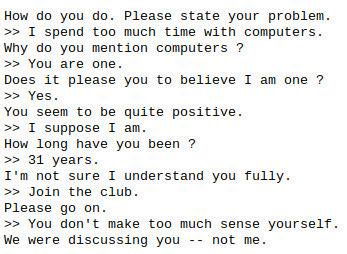
\includegraphics[width=5cm]{figuras/eliza}
\caption{\label{fig:eliza}Exemplo de um dialogo entre Eliza e seu terapeuta}
\end{figure}

\emph{Eliza}, entretanto, não é um exemplo de ficção Interativa. Acontece que o
programa não simula universo algum, e não parece ter uma boa compreensão do que
fala a personagem. Ainda sim, o programa resguarda a sua importância histórica
para o mundo da FI no fato de representar o primeiro uso \footnote{conhecido} do
modelo de interação entre humanos e máquinas que seria replicado nas primeiras
aventuras de texto. Alguns desses primeiros jogos terminavam cada turno
perguntando ao jogador o que fazer, e respondiam a uma falha de compreensão
dizendo que não era possível fazer aquilo (o que quer que fosse). Isso é um
traço herdado desse programa piloto. Não se trata de uma prática muito
recorrente nos dias atuais, mas ajuda a visualizar a evolução desse tipo de
software.

Depois de \emph{Eliza}, temos \emph{Kill the Wumpus} (1972) como uma
representação mais próxima do que podemos chamar de ficção interativa. Nessa
aventura, o personagem central explora uma rede de cavernas e tem a missão de
matar uma criatura terrível, cuja descrição pode ser vaga, mas seu poder letal é
muito concreto.

O jogo desenvolve-se numa narrativa que passa por entre os cenários conectados
por passagens. O jogo nos diz onde estamos, e onde podemos ir a partir de lá.
Não há interpretador, e tudo o que o jogador pode fazer é atirar uma flecha ou
sair dali. Veja um exemplo abaixo.

\begin{figure}[htb]
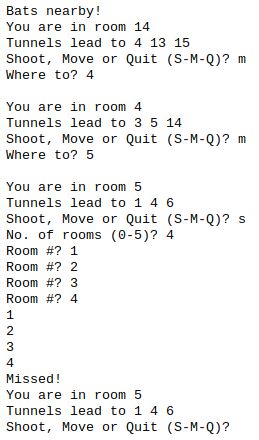
\includegraphics[width=5cm]{figuras/wumpus}
\caption{\label{fig:wumpus} \emph{Gameplay} do jogo Kill the Wumpus}
\end{figure}

O maior desafio desse jogo provavelmete resida no fato da personagem ter que usar
de alguns subterfúgios para enfrentar a besta. Confronto geral acabava com a
inevitável morte da personagem. Vencer no jogo significa explorar bem o meio
enquanto tenta evitar Wumpus. Por sorte, podemos sentir o cheiro da besta quando
estamos por perto. Mas tal "ajuda" contrapõe-se com outras dificuldades. É um
jogo que requer um certo nível de lógica.

Ainda que o jogo pareça bastante primitivo, ele representa um grande passo para o
que hoje chamamos de ficção interativa. É um avanço e tanto se consisderarmos
\emph{Eliza}. Enquanto o primeiro responde apenas ao último input do jogador,
\emph{Kill the Wumpus} trata de simular um mundo dentro da memória da máquina,
ainda que este mundo seja limitadíssimo. Cada passo e ação tinha uma ação
permantente no estado do jogo.

O jogo é um desafio de localização, e muitas aventuras de texto levaram bastante
a sério a geografia na hora de produzir os desafios. Esse movimento foi tão
forte, que quase toda ficção interativa viu-se obrigada a incluir um conjunto de
labirintos, quanto mais bagunçados, melhor. Em alguns casos, a organização, ou a
falta dela era tamanha que ir pro norte e depois pro sul imediatamente depois não
te levaria de volta ao mesmo lugar. Segundo o autor, por alguma razão, esses
labirintos, se fossem planejados de forma linear, eram mal vistos e tidos como
anti exemplos do que se esperava desse gênero de aventura
% busy-work << trabalho cotidiano que gera mais cansaço que resultado

Um tempo depois, levado pela vontade de agradar suas filhas pequenas,
com as quais ele passava pouco tempo, sua paixão pela geologia, e habilidades de
programação, Will Crowther criou \emph{Adventure}. O jogo utiliza dos seus
conhecimentos sobre cavernas, e é influenciado pelo jogo
\emph{Dungeons and Dragons} no uso de mágicas pelo personagem. A princípio, o
jogo fora pensado exclusivamente para o divertimento de suas filhas, mas chegou
em pessoas como Dom Woods que, impressionado com o jogo, disse:
\begin{quotation}
\emph{Adventure} fez usuários pensarem que estavam interagindo mais com o
computador. (...) Parecia que respondia melhor ao que se escrevia, ao invés de
fazer seus próximos movimentos, tal como um omponente silencioso. Acredito que
tenha atraído muitos jogadores que se desligaram da ideia de jogar
\textbf{contra} o computador. Tratava-se, pois, de jogar \textbf{com} a máquina.
\end{quotation}

Maravilhado com o trabalho que encontrou, Woods contata Crowther para poder
polir e destribuir o jogo que Will havia criado. Depois do trabalho concluído,
acrescenta-se uma "pitada" de Token. A aventura se resume a coletar os tesouros
de uma caverna, e levá-los em segurança pra superfície. Isso é claro, enquanto
enfrenta trolls, elfos e outras criaturas.

\begin{figure}[htb]
  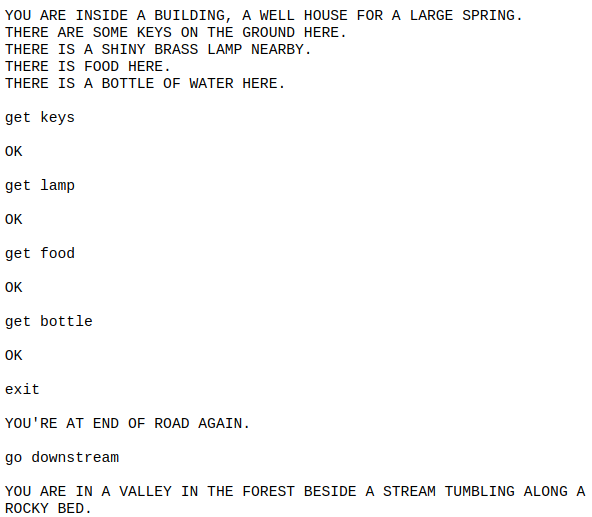
\includegraphics[width=5cm]{figuras/adventure}
  \caption{\label{fig:adventure} \emph{Gameplay} do jogo Adventure}
\end{figure}

Ainda que o jogo tenha uma série de defeitos, como puzzles sem nexo, e mortes
inesperadas, saber dele nos torna mais conscientes, da evolução da FI. Cada um
desses trabalhos traz consigo pontos de evolução em relação às limitações dos
demais. Tais limitações, entretanto, leva-nos a enxergar o caminho todo sob
um prisma muitas vezes distinto do que se via na ocasião. Não podemos ignorar
que o público da época era bem menos exigente\footnote{não entenda como
condescendência, pois os padrões técnicos, advindos do estágio de avanços
tecnlógico, eram distintos}, e tinha outras excpectativas com relação a esse tipo
de software. Alguns dos traços, que o mundo da IF enxerga como defeitos,
antigamente não o eram.

De certo, houveram muitos outros percussores, e parte desses não serão
conhecidos, mas o mais belo é imaginar que parte desses personagens, bem como
outros tantos desconhecidos, não tinham a pretenção de terem seus nomes guardados
na história. Motivo de tal creça parte do fato de que, nas décadas de 60 e 70, o
computador não gozava da popularidade e acessibilidade que tem hoje, e a
profissão de programador não tinha o glamour que tem hoje, e o alcance das obras
também era bem menor.

Há muitas reflexões muito convenientes para se fazer a respeito da história da
Ficção Interativa, entretanto uma exploração mais profunda seria um grave desvio
a proposta inicial. Desejava-se, com essa explicação, colocar em contexto o que
foi apresentado no passado, para entender o que será feito nesse trabalho, e o
que já foi feito.

\subsection{ZIL, Inform e outras ferramentas}
\label{subsec:tools}

Essa parte do trabalho tem como única função, apresentar algumas ferramentas com
o mesmo intuito que aquela que estou preparando. A apresentação será rápida, já
que o foco não está nessas ferramentas, e sim no que elas influenciam os demais
criadores e a esse trabalho.

ZIL\footnote{Zork Implementaion Language} foi a linguagem usada pela Infocom e
originou-se a partir de MDL \footnote{também chamado de "muddle"} durante o
processo de criação de Zork. O processo que levou a sua criação é um evento muito
interessante, mas como não é o foco dessa análise, recomendo a leitura do
capítulo 4 de \citep{Jim:06} \footnote{sessão \textbf{The Birth Of Infocom and
The Zork Trilogy}}.

A linguagem "pai", MDL\footnote{MIT Design Language} foi criada pelo grupo do
Laboratório de Ciência da Computação (LCS) daquela universidade, dirigida por
outras necessidades alheias à empreitada de escreverem seus próprios jogos. Quando
tal ímpeto surgiu nos participantes daquele grupo, a primeira ideia foi usar
aquela ferramenta, inspirada na linguagem LISP que eles já conheciam. Para
economizar recursos de máquina (que já estavam rompendo a barreira do disponível
durante a produção do jogo \emph{Zork}), decidiram por remover do MDL o que não
era necessário à produção do jogo. Possivelmente tenha sido a primeira linguagem
a ser criada com esse intúito específico. A linguagem mantem uma aparência muito
parecida com LISP, da qual foi gerada indiretamente. Tal fenômeno não é uma
surpresa, dado que MDL fora criado com base em LISP, e que ZIL, a grosso modo,
não seria mais que uma versão enxuta de MDL.

\begin{figure}
  \centering
  \subfloat[LISP \cite{LISP}]{{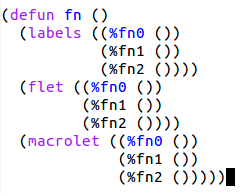
\includegraphics[width=.2\textwidth]{figuras/lisp}}}
  \subfloat[MDL \cite{MDL}]{{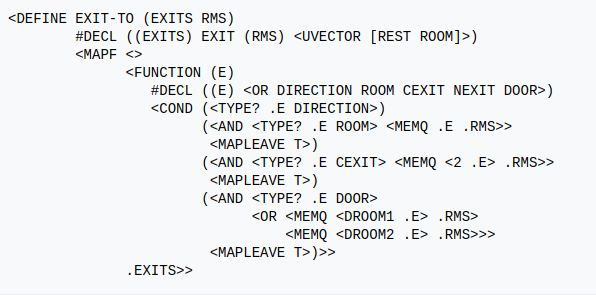
\includegraphics[width=.35\textwidth]{figuras/mdl}}}
  \subfloat[ZIL \cite{IF3}]{{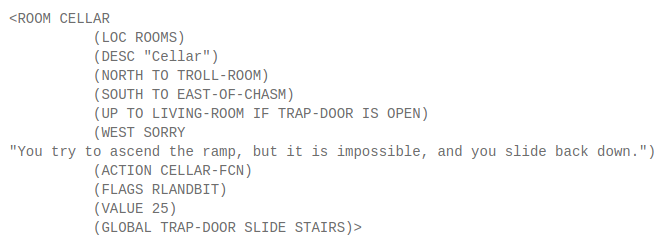
\includegraphics[width=.45\textwidth]{figuras/zil}}}
  \caption{Exemplo das linguagens mencionadas}
  \label{fig:zil}
\end{figure}

Além do ZIL, temos também outras ferramentas pra produção desse tipo. A título
de exemplo temos Inform e o TADS \footnote{Text Adventure Development System}.
As duas surgiram na década de 90, e cada uma tem suas características próprias.
Ambas tornaram-se opções viáveis ao ZIL. TADS é baseada em C, que naquela década
teve seu pico de popularidade, e sua evolução foi majoritariamente voltada à sua
implementação. Inform, por outro lado, é uma linguagem procedural, e sua
evolução teve alicerce nos estudos de seus próprios criadores sobre linguagem
natural \footnote{vide artigo \citet{Nel:06}}. Na figura \ref{fig:other-tools},
tratei de inserir imagens para que se possa visualizar um pouco das
características mencionadas acima.

\begin{figure}
  \centering
  \subfloat[Inform7 \cite{Inf7}]{{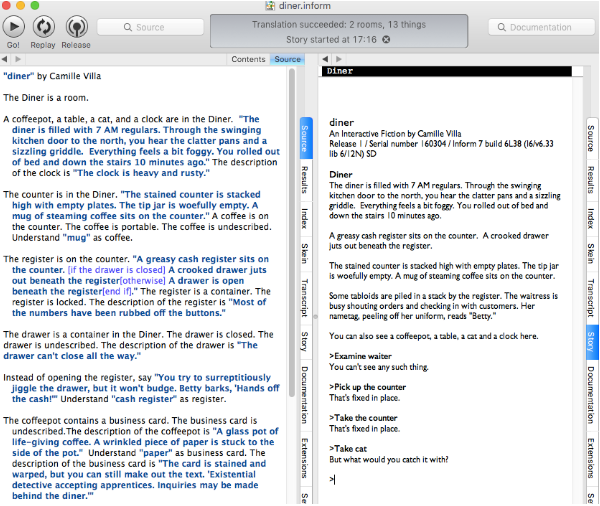
\includegraphics[width=.3\textwidth]{figuras/inform}}}
  \subfloat[TADS \cite{Eve:12}]{{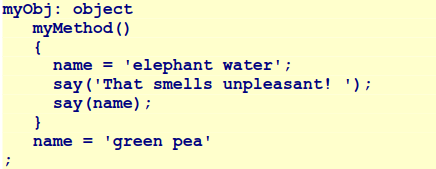
\includegraphics[width=.5\textwidth]{figuras/TADS}}}
  \caption{Exemplos de Inform7 e TADS}
  \label{fig:other-tools}
\end{figure}

Tendo tratado da história da Ficção Interativa e das ferramentas mais conhecidas,
o próximo passo é tratar da linguagem escolhida para fazer a implemetação.

\section{Ruby}
\label{sec:ruby}

Ruby é uma linguagem de programação orientada a objetos criada por Yukihiro
Matsumoto em 1993. Ruby pode ser considerada como que um encontro entre Python,
Perl e Smalltalk. Por ser uma linguagem tão versátil e permitir que o
desenvolvedor concentre melhor suas energias em fazer o algoritmo \footnote{ao
invés de ficar lutando contra a programação}  como disseram \citet{Rcook:09}, e
por outros motivos, escolheu-se Ruby para o desenvolvimento.

Ruby apresenta uma notável facilidade em lidar com expressões regulares, fator
de grave importância para a produção do interpretador. Além disso, programar em
Ruby é um exercício menos cansativo do que boa parte das outras linguagens,
muito em razão de alguns de seus métodos ou palavras chaves tornarem o texto do
arquivo fonte mais compreensível para humanos e máquinas exercitando a sugestão
de D. E. Knuth que recomenda que a programação deva ser feita de modo que
humanos entendam o que se pediu da máquina. Um arquivo bem formatado em Ruby
permite que tal recomendação seja posta em prática. Veja, na figura
\ref{fig:ruby} um exemplo tirado do mesmo livro que foi citado no parágrafo
acima e que serve de fonte para esse trabalho. Em caso de necessidade de uma
consulta mais rápida, o site
\href{https://www.tutorialspoint.com/ruby/index.htm}{\textbf{Tutorials Point}}
também é uma boa sugestão.

\begin{figure}
  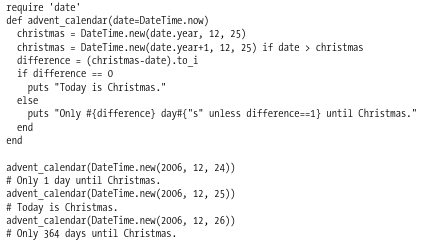
\includegraphics[width=10cm]{figuras/ruby}
  \caption{Exemplo de função escrita em ruby}
  \label{fig:ruby}
\end{figure}

\section{RSpec}
\label{sec:rspec}

Para produzir os testes que garantem, na medida do possível a consistência e o
funcionamento completo do programa, esse projeto usa RSpec. Diferentemente de
outras ferramentas de teste, o seu foco é no comportamento das funções como
podemos observar na figura \ref{fig:rspec}. Trata-se da ferramenta mais adequada
por garantir que os métodos a serem desenvolvidos seguirão o comportamendo
esperado.

\begin{figure}[htb]
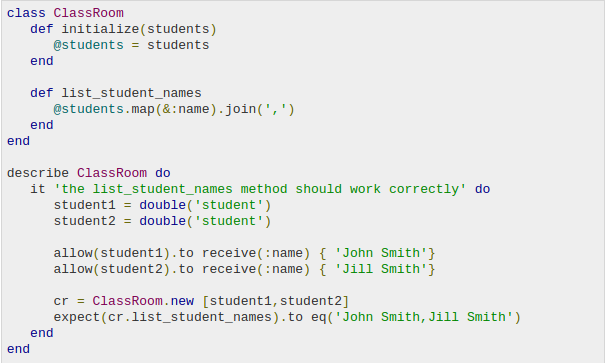
\includegraphics[width=10cm]{figuras/rspec}
\caption{\label{fig:rspec} Exemplo de programa e teste respectivo}
\end{figure}

Mais do que uma ferramenta de testes, RSpec também foi adotado por mim como
modelo de implementação para o sistema de criação de FI's. Cada elemento,
quarto, personagem, objeto será descrito através de pares chave e valor, a serem
embrulhadas por declarações como: \textbf{\texttt{Objeto Mesa tem ... fim}} ou
\textbf{\texttt{Objeto Mesa \{ ... \} }}. Tal decisão se apoia sob a hipótese (a
ser testada) de ser a mais intuitiva.
